\documentclass[conference]{IEEEtran}
\IEEEoverridecommandlockouts
\usepackage{cite}
\usepackage{amsmath,amssymb,amsfonts}
\usepackage{algorithmic}
\usepackage{graphicx}
\usepackage{textcomp}
\usepackage{xcolor}
\usepackage{hyperref}
\usepackage{booktabs}

\def\BibTeX{{\rm B\kern-.05em{\sc i\kern-.025em b}\kern-.08em
    T\kern-.1667em\lower.7ex\hbox{E}\kern-.125emX}}

\begin{document}

\title{PhishGuard: A Multi-Feature Machine Learning Framework for Phishing URL Detection}

\author{\IEEEauthorblockN{Md. Akram Hossain Khandoker Himel \\ Toyhid Shikder }
\IEEEauthorblockA{\textit{ Department of Computer Science and Engineering } \\
\textit{ Green University of Bangladesh }\\
}
}

\maketitle

\begin{abstract}
Phishing attacks remain one of the most prevalent cybersecurity threats, with attackers continuously evolving their techniques to evade detection. This paper presents PhishGuard, a comprehensive machine learning framework for detecting phishing URLs by leveraging multiple feature sets: WHOIS information, SSL certificate data, and behavioral characteristics. Our approach combines these diverse feature sets to create a robust detection system that achieves high accuracy while maintaining resilience against evasion techniques. Experimental results demonstrate that our Random Forest model utilizing all feature sets achieves 99.52\% accuracy, outperforming models trained on individual feature sets. We also provide a comparative analysis of Random Forest and XGBoost algorithms across various feature combinations, highlighting the strengths of each approach. The framework's modular design allows for graceful degradation when certain features are unavailable, making it practical for real-world deployment scenarios.
\end{abstract}

\begin{IEEEkeywords}
Phishing Detection, Machine Learning, WHOIS, SSL Certificates, URL Features, Random Forest, XGBoost
\end{IEEEkeywords}

\section{Introduction}
Phishing is a strategy for cyber crime. Where the attacker use false websites, email or message to attack the normal random users to get their name, address, passwords or other personal information \cite{wikipedia2025phishing}. In recent days, the number of phishing attacks are increasing. In the current scenario, implementing a phishing attack is very easy and also profitable financially\cite{wired2021aipishing}. In many research, we can see that for breaking cyber security the phishing is the most common reason\cite{oni2024phishing}. So, making a flexible and working phishing detection is very important in the world. \\

For detecting current running phishing websites we used blacklist and whitelist system \cite{academia2022mlphishing}. But, this type of systems can not work for digital phishing websites. Because attacker update their mathod regularly. They update their domain name, change url structure also copy the legit ssl certificates. Those informations are not available in the blacklist \cite{sciencedirect2022noveldataset}. For these type of challenges by using machine learning algorithm, the trend of making a phishing detection system has increased \cite{mdpi2022improved, academia2020cnn}. \\ 

ML-based phishing detection systems generally leverage three categories of features: (1) WHOIS-based domain attributes such as domain age, registrar details, and ownership privacy \cite{academia2024survey}; (2) SSL certificate metadata, including issuing authority, certificate validity period, and cryptographic properties \cite{mdpi2023deeplearning}; and (3) behavioral features, such as webpage content, URL structures, JavaScript activity, and redirection patterns \cite{futureinternet2022behavior}. While models trained on a single feature group often struggle with misclassification, combining multiple feature categories has been shown to significantly improve detection accuracy \cite{frontiers2025multimodal}. \\

However, high accuracy alone is not sufficient. Recent studies highlight that black-box models, such as deep neural networks, often fail to provide interpretability or explainability \cite{wiley2022explainable}. As a result, cybersecurity professionals cannot always understand why and how a model arrives at its decision. To overcome this limitation, hybrid models, feature importance analysis \cite{arxiv2024featureimportance}, and explainable AI methods are increasingly being explored to balance performance with transparency. \\

The primary goal of our research is to design a multi-layered phishing detection framework that integrates WHOIS, SSL, and behavioral features in a unified system. Separate machine learning models will be trained for each feature group, and a dynamic combination mechanism will be applied to produce the final prediction. This ensures robustness in real-world conditions—if certain feature groups are missing (e.g., SSL data unavailable), the framework can still generate reliable predictions. This approach addresses a major gap in existing studies, which often assume the availability of complete datasets \cite{academia2021urltran, irep2025benchmarking}. \\

Therefore, machine learning–based phishing detection is no longer confined to academic research but is rapidly evolving into a practical security tool for real-world applications \cite{wikipedia2025applicationsAI}. Our proposed framework, with its multi-layered design and flexible feature handling, can be extended into practical solutions such as browser extensions or network-level defenses, contributing significantly to strengthening digital security. 

\section{Related Work}
Several studies have addressed phishing detection using a variety of approaches. Initially, blacklist and whitelist techniques were employed to identify new phishing domains \cite{academia2022mlphishing}. However, these rule-based methods proved ineffective for newly registered or previously unseen domains \cite{sciencedirect2022noveldataset}.

In recent years, machine learning–based approaches have demonstrated significant effectiveness. For example, Random Forest and XGBoost models have been applied to URL, WHOIS, and SSL feature analysis to detect phishing websites \cite{oni2024phishing, mdpi2022improved}. Additionally, deep learning techniques such as CNNs and LSTMs have successfully analyzed webpage content and user behavior for phishing detection \cite{academia2020cnn}.

Some studies have combined multiple feature groups to train models. For instance, WHOIS + SSL + Behavioral features have been used together with multiple ML models and combination strategies \cite{frontiers2025multimodal, academia2021urltran}. This multi-feature approach overcomes the limitations of single-feature models and achieves higher prediction accuracy.

However, accuracy alone is not sufficient. Explainable AI (XAI) methods are increasingly important to provide interpretable predictions \cite{wiley2022explainable, arxiv2024featureimportance}. Such interpretability enhances trust for cybersecurity experts and improves practical applicability in real-world scenarios.

Recent research has also explored URL transformers and multimodal frameworks to advance phishing detection \cite{academia2021urltran, frontiers2025multimodal}. Our proposed framework is built on a similar hybrid and dynamic combination approach, leveraging multiple feature groups for robust and explainable phishing detection.


\section{Methodology}
The PhishGuard framework is designed as a multi-layered system consisting of four key components: dataset preparation, feature extraction, feature processing, and model training with prediction. Figure \ref{fig:methodology} illustrates the overall architecture of our system.

\begin{figure}[htbp]
\centerline{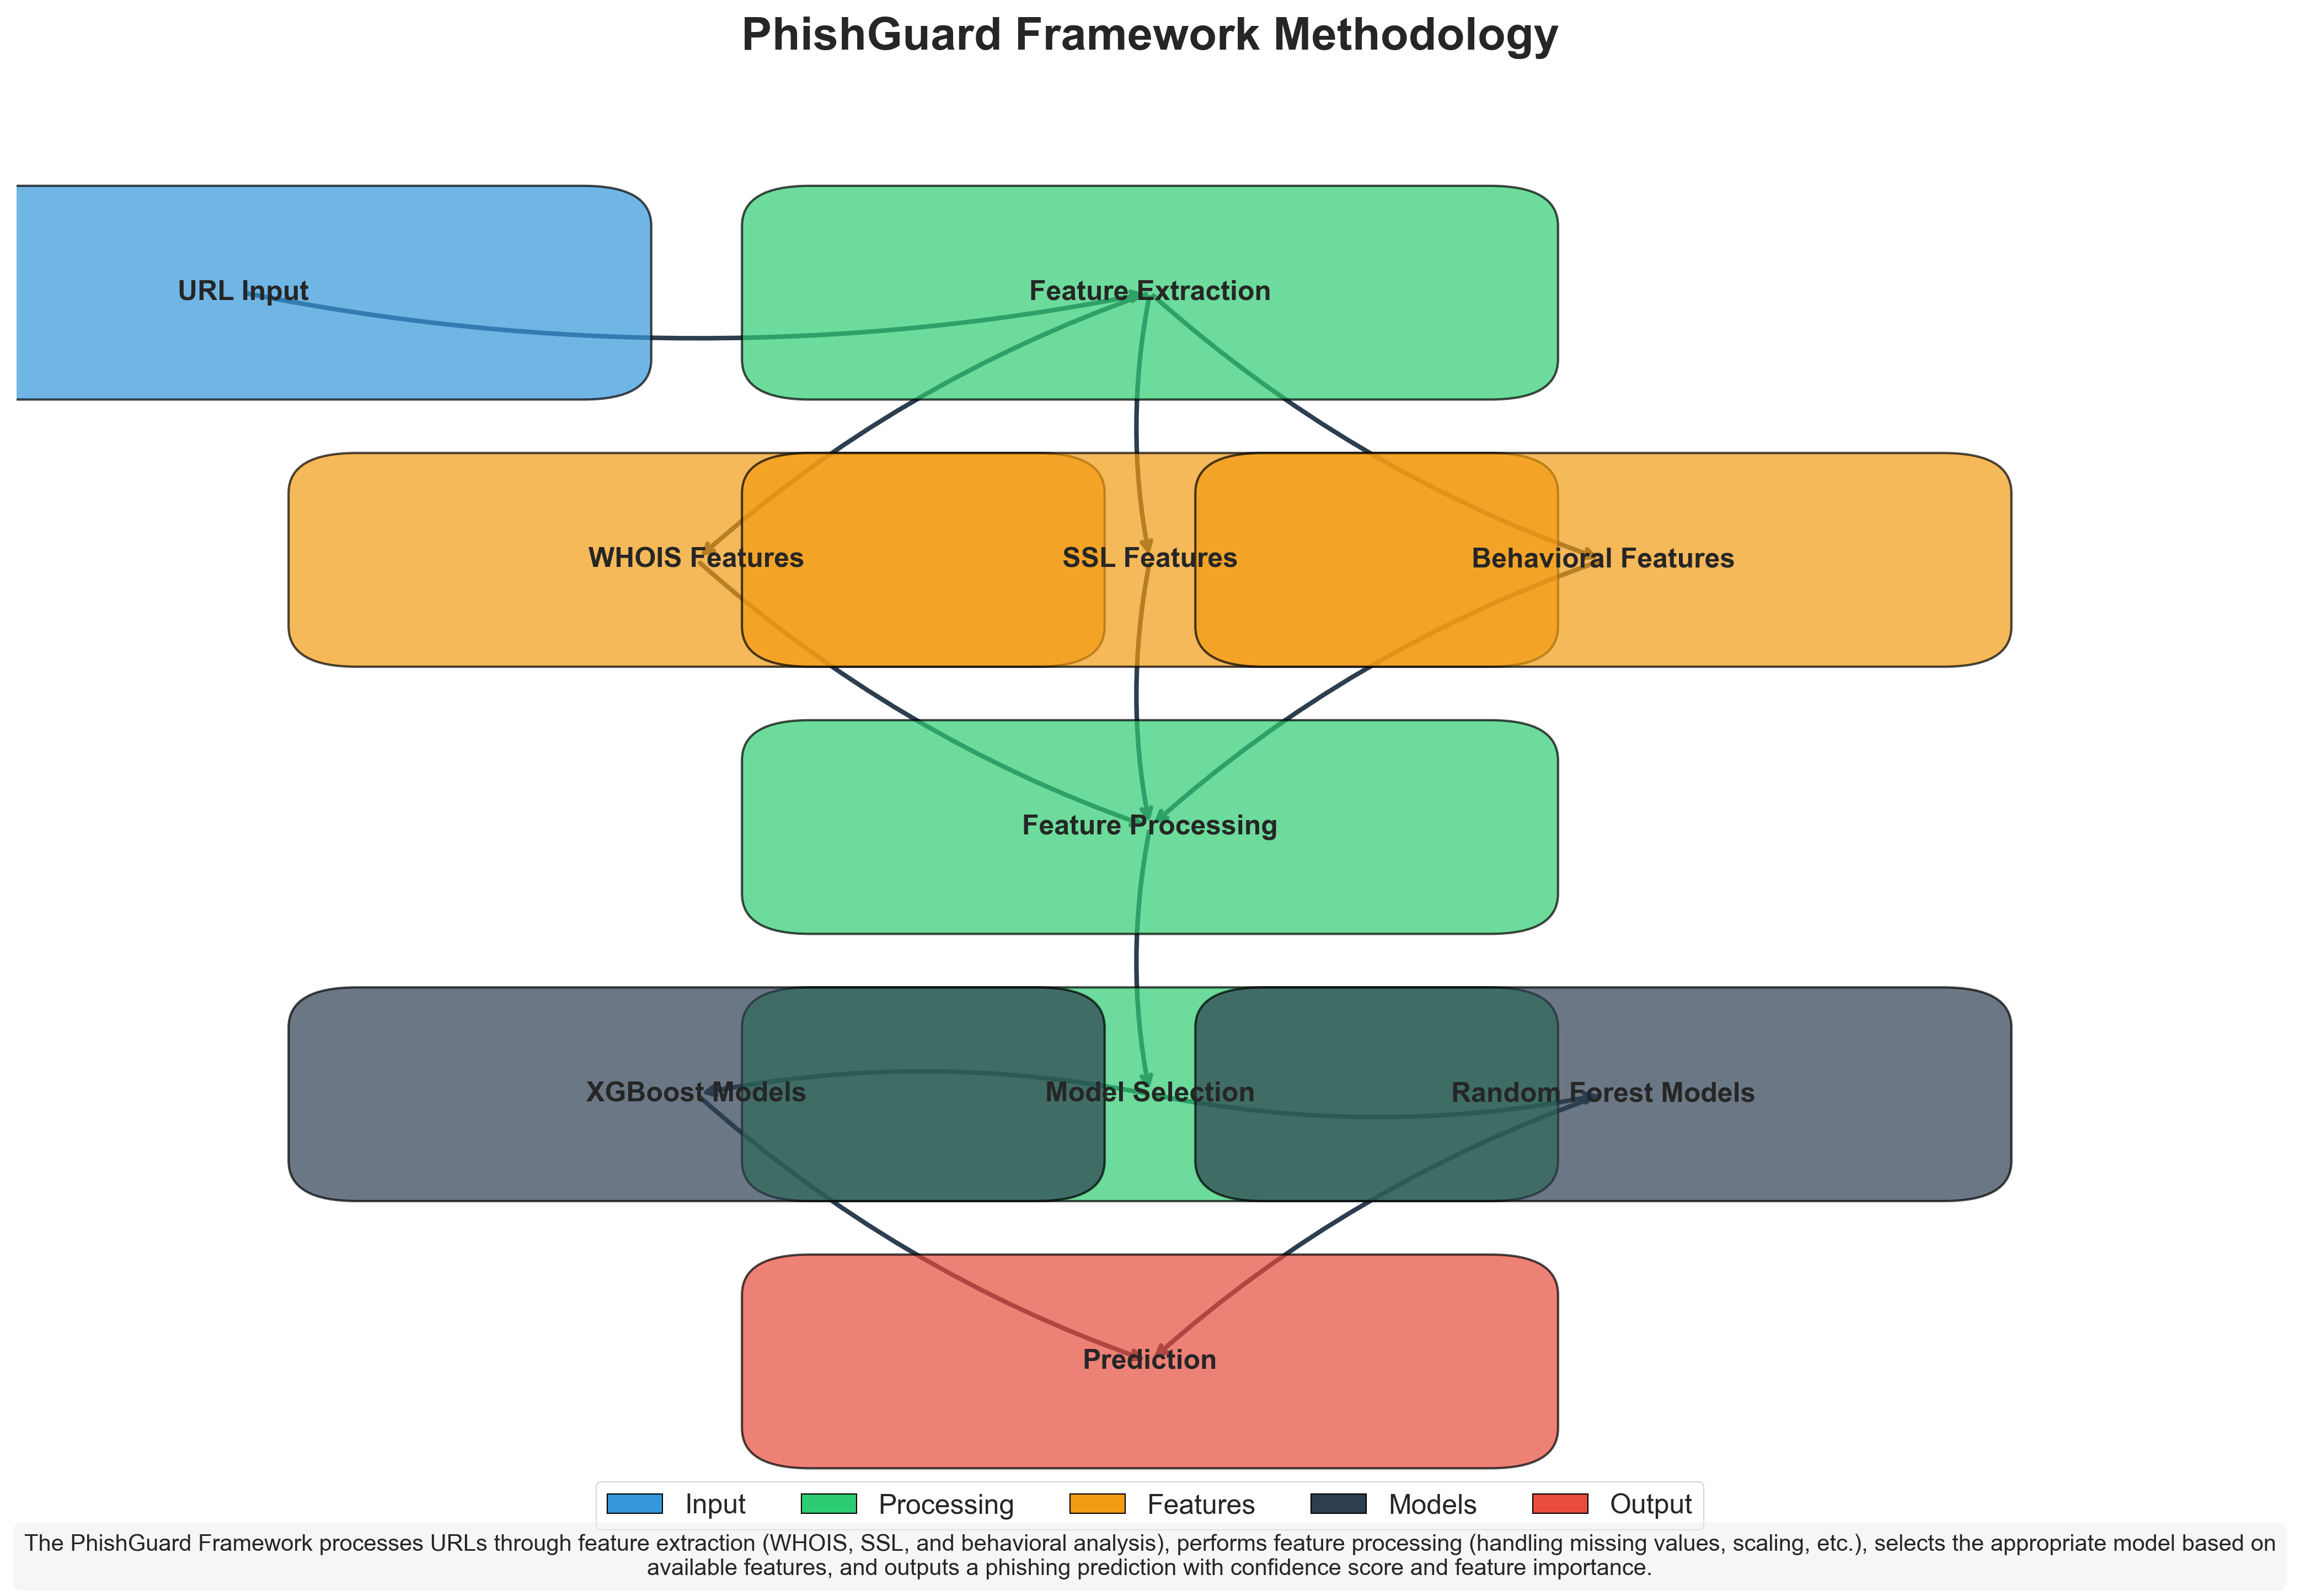
\includegraphics[width=0.9\columnwidth]{image/methodology_diagram.png}}
\caption{PhishGuard Framework Architecture}
\label{fig:methodology}
\end{figure}

\subsection{Dataset}
Our dataset consists of 1,031 URLs, including 849 phishing sites and 182 legitimate websites. The legitimate URLs were collected from Alexa's top-ranked websites, ensuring trustworthiness and coverage across multiple domains such as banking, e-commerce, and social networking \cite{sciencedirect2022noveldataset}. Phishing URLs were gathered from reliable public repositories such as PhishTank and OpenPhish, which are widely adopted in academic research \cite{academia2022mlphishing}. This balanced yet diverse dataset design is consistent with prior works in phishing detection \cite{systlitchange2023, oni2024phishing}.

\subsection{Feature Extraction}
The PhishGuard framework extracts three categories of features: WHOIS-based, SSL certificate–based, and behavioral attributes. These features were selected based on their proven discriminative power in phishing detection research \cite{futureinternet2022behavior, mdpi2022improved, acm2024features}.

\textbf{WHOIS Features:} WHOIS information provides critical temporal and administrative details of domain registration, which have been widely linked with phishing activity \cite{systlitchange2023}. Features include:
\begin{itemize}
    \item Domain age (registration date)
    \item Expiration date
    \item Last update date
    \item Registrar information
    \item Country of registration
    \item Privacy protection status
\end{itemize}

\textbf{SSL Certificate Features:} Malicious websites often misuse or forge SSL certificates. As demonstrated in prior work \cite{mdpi2022improved}, analyzing certificate details enhances phishing detection accuracy. Extracted features include:
\begin{itemize}
    \item Certificate validity period
    \item Issuer information
    \item Certificate algorithm
    \item Self-signed status
    \item Certificate age
\end{itemize}

\textbf{Behavioral Features:} User-facing attributes of URLs and domain structures provide important signals of phishing intent \cite{futureinternet2022behavior, academia2020cnn}. The behavioral features include:
\begin{itemize}
    \item URL length
    \item Number of subdomains
    \item Number of special characters
    \item Presence of IP address
    \item Domain popularity
    \item Presence of suspicious TLDs
    \item Presence of suspicious keywords
    \item Redirect count
\end{itemize}

To improve robustness, the framework implements error-handling mechanisms in cases where certain features are unavailable (e.g., protected WHOIS records or expired SSL certificates), as also recommended in prior studies \cite{acm2024features}.

\subsection{Feature Processing}
The extracted features undergo structured preprocessing before model training. Preprocessing is essential since phishing datasets often contain missing values and heterogeneous data types \cite{academia2024survey}.

\begin{enumerate}
    \item \textbf{Handling categorical variables:} Categorical attributes (registrar, country, SSL issuer, algorithm) were encoded using one-hot encoding to ensure compatibility with ML models \cite{oni2024phishing}.
    \item \textbf{Date processing:} Temporal values (e.g., domain age) were transformed into numerical representations (days since registration).
    \item \textbf{Missing value imputation:} Missing values were replaced using context-specific defaults or median values to avoid bias.
    \item \textbf{Feature scaling:} Continuous features were standardized using the StandardScaler method to balance the contribution of features \cite{mdpi2022improved}.
\end{enumerate}

\subsection{Model Training}
We evaluated two machine learning algorithms that have consistently demonstrated strong performance in phishing detection \cite{irep2025benchmarking, academia2022mlphishing}:  

\begin{enumerate}
    \item \textbf{Random Forest:} An ensemble method that constructs multiple decision trees and outputs the mode class of individual predictions. Its robustness against overfitting makes it suitable for phishing detection tasks \cite{oni2024phishing}.
    \item \textbf{XGBoost:} A gradient boosting framework optimized for speed and performance. Its regularization capabilities reduce overfitting and improve generalization \cite{mdpi2023deeplearning}.
\end{enumerate}

Each algorithm was trained on multiple feature set combinations to evaluate the discriminative power of different categories:
\begin{itemize}
    \item WHOIS features only
    \item SSL features only
    \item Behavioral features only
    \item WHOIS + SSL features
    \item WHOIS + Behavioral features
    \item SSL + Behavioral features
    \item Combined (all features)
\end{itemize}

We adopted a stratified 5-fold cross-validation approach to ensure robust and fair evaluation while preserving the ratio of legitimate and phishing samples across folds \cite{systlitchange2023}. To address class imbalance, class weights inversely proportional to class frequencies were applied during training, following practices in prior phishing detection studies \cite{academia2024survey, wiley2022explainable}.


\section{Results and Evaluation}

\subsection{Model Performance Comparison}
Figure \ref{fig:rf_comparison} shows the performance comparison of Random Forest models across different feature sets.

\begin{figure}[htbp]
\centerline{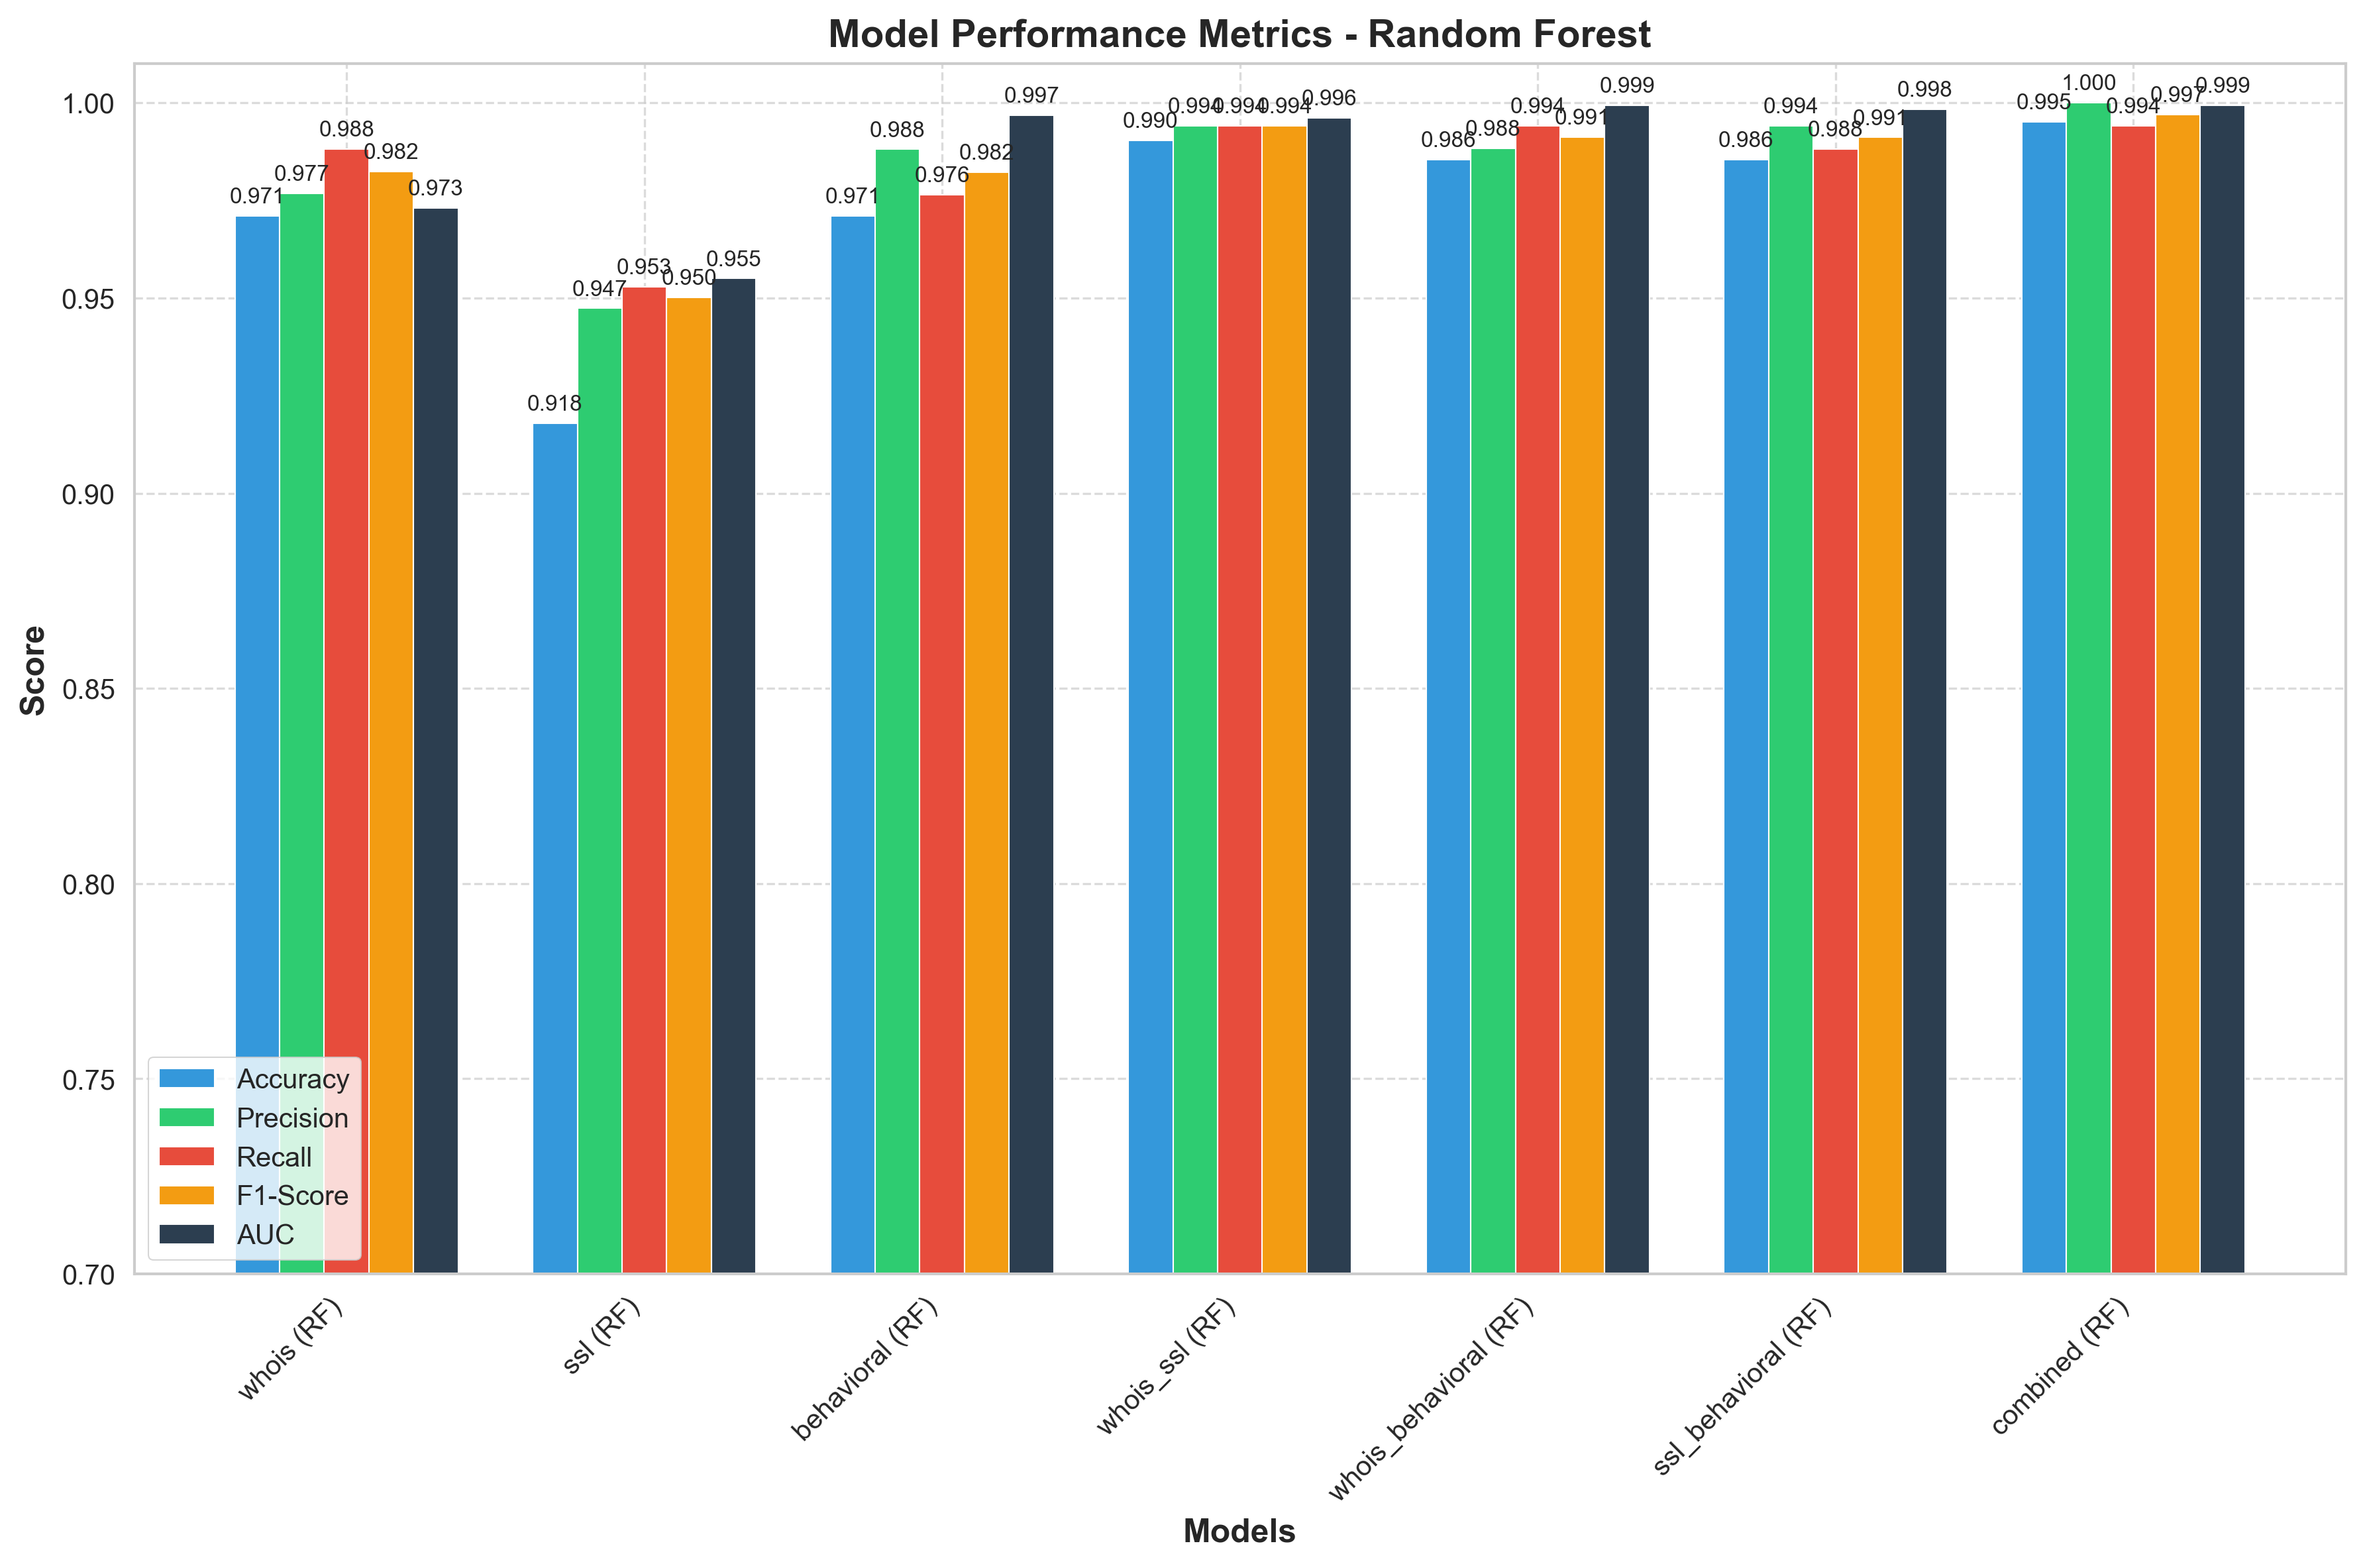
\includegraphics[width=0.9\columnwidth]{image/model_comparison_random_forest.png}}
\caption{Performance Metrics for Random Forest Models}
\label{fig:rf_comparison}
\end{figure}

Figure \ref{fig:xgb_comparison} presents the performance comparison of XGBoost models across different feature sets.

\begin{figure}[htbp]
\centerline{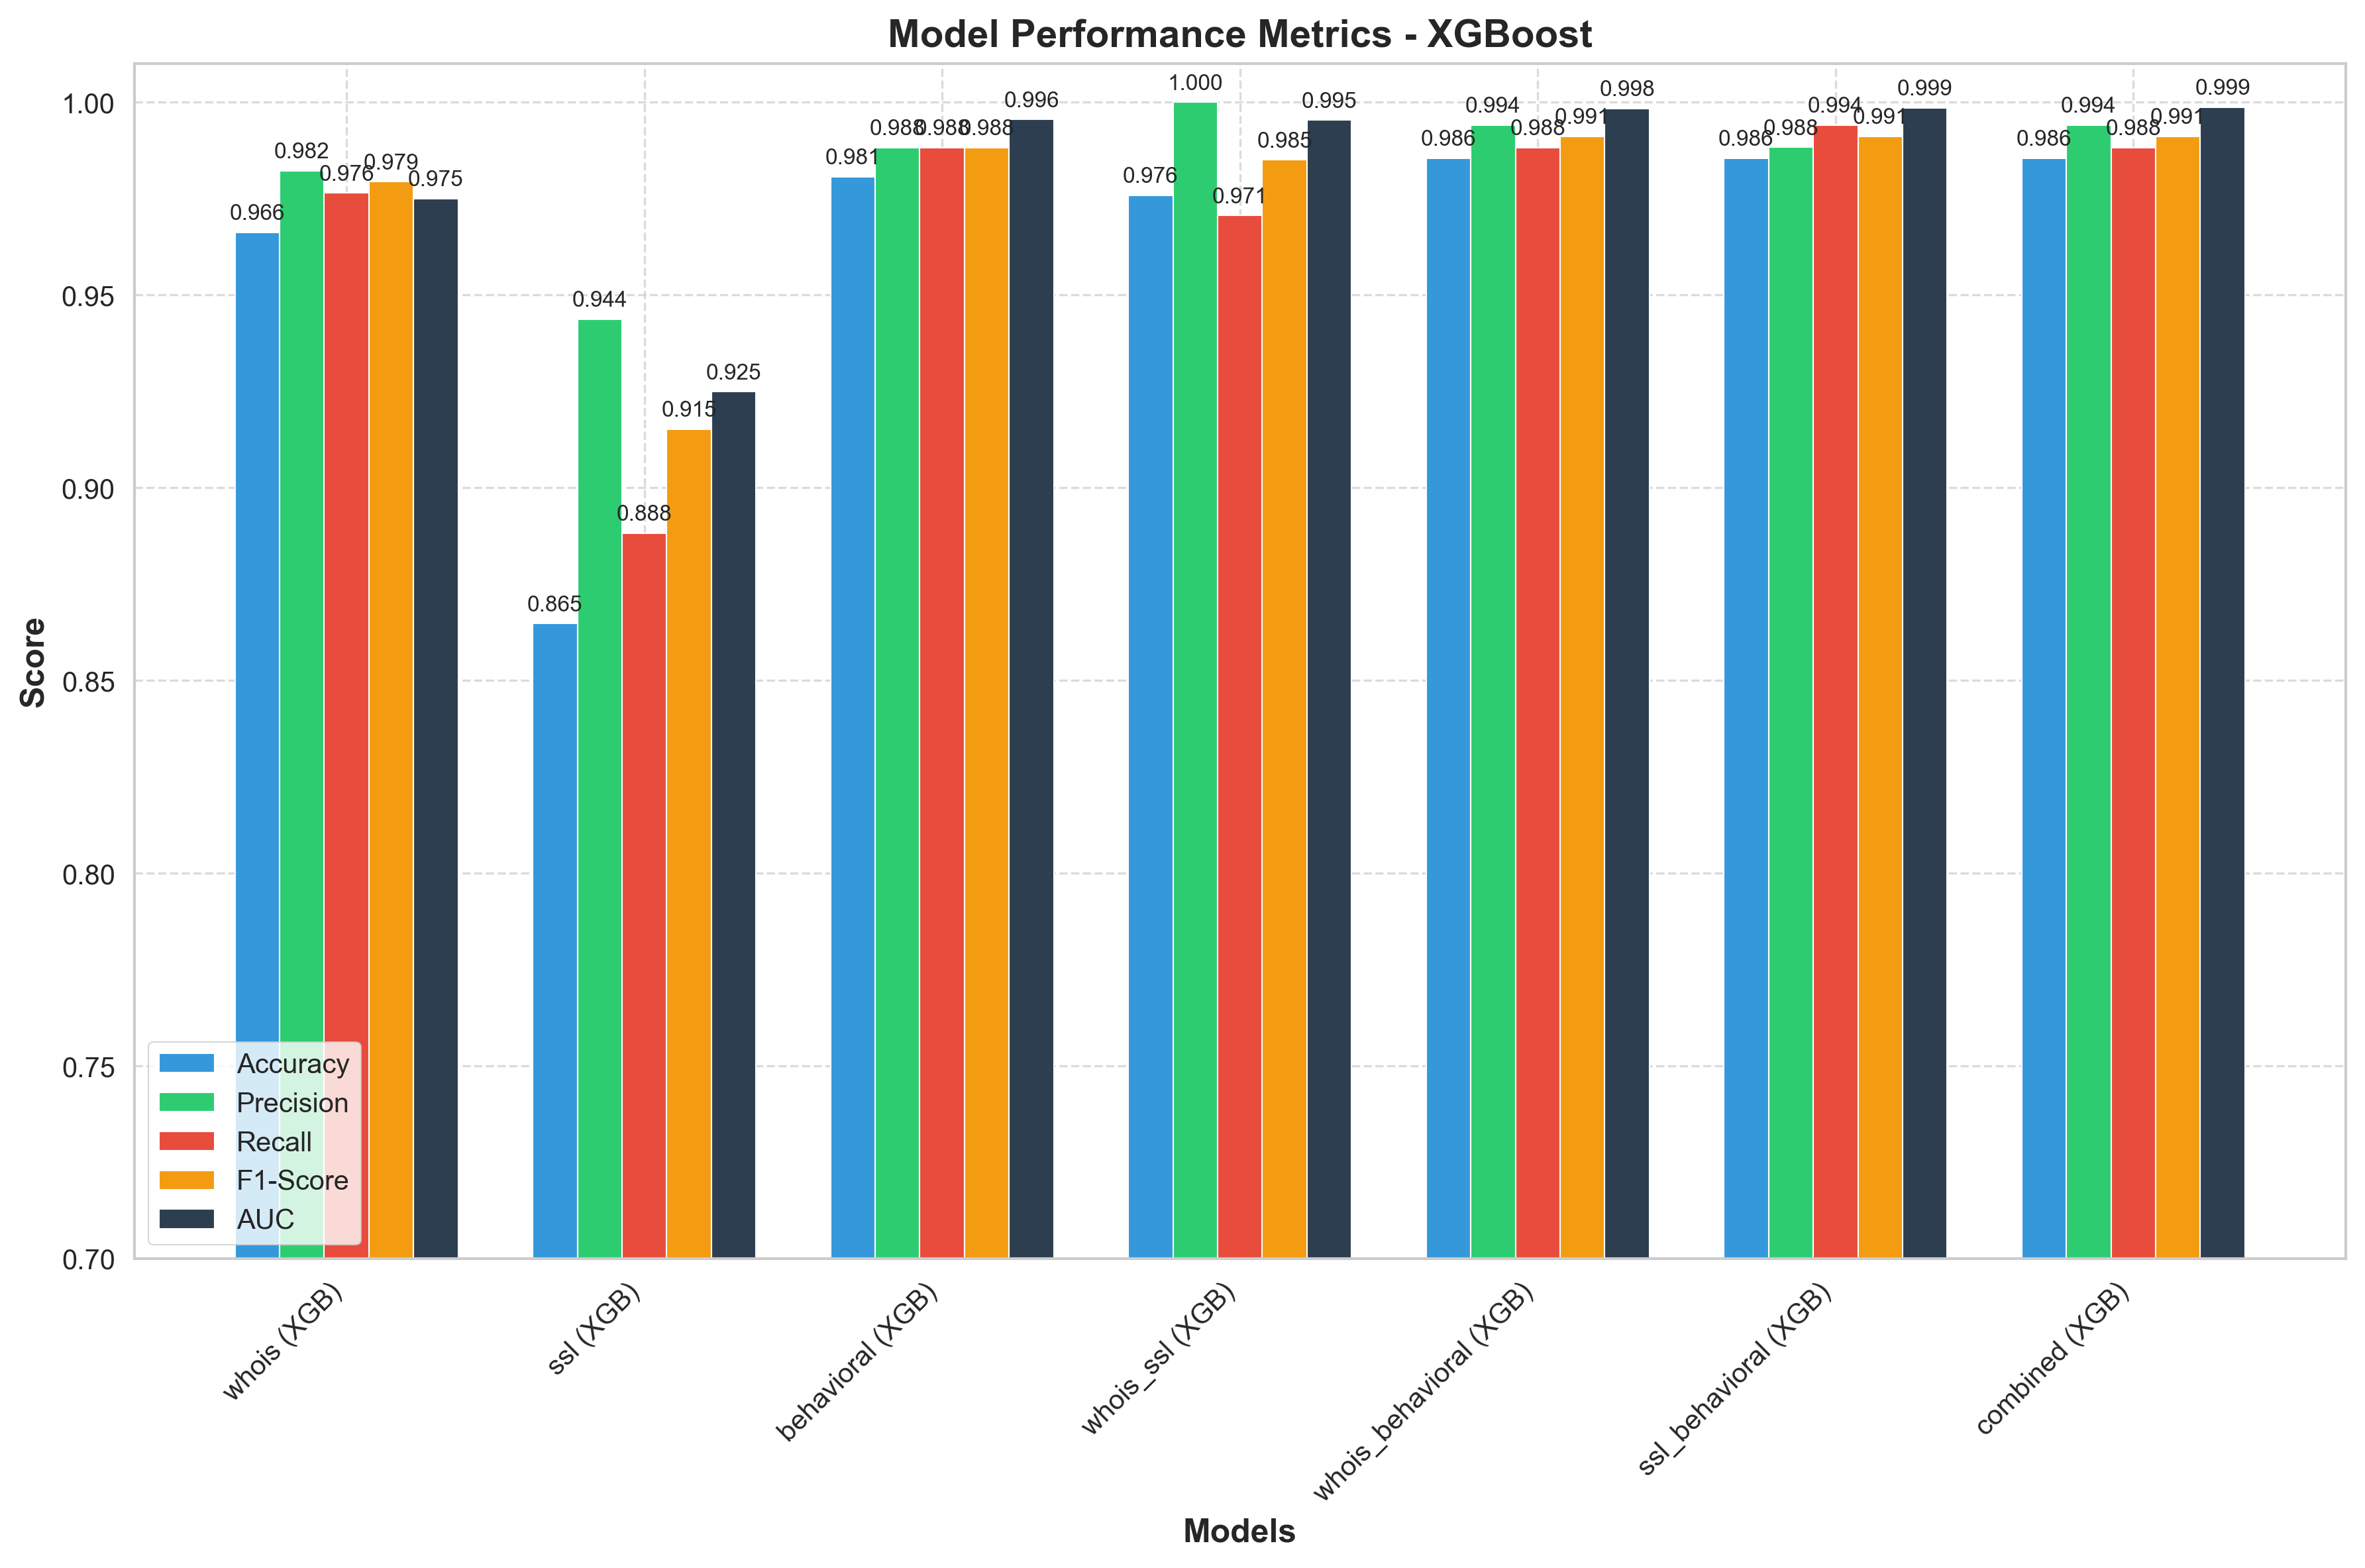
\includegraphics[width=0.9\columnwidth]{image/model_comparison_xgboost.png}}
\caption{Performance Metrics for XGBoost Models}
\label{fig:xgb_comparison}
\end{figure}

Figure \ref{fig:best_models} compares the best-performing models from each algorithm.

\begin{figure}[htbp]
\centerline{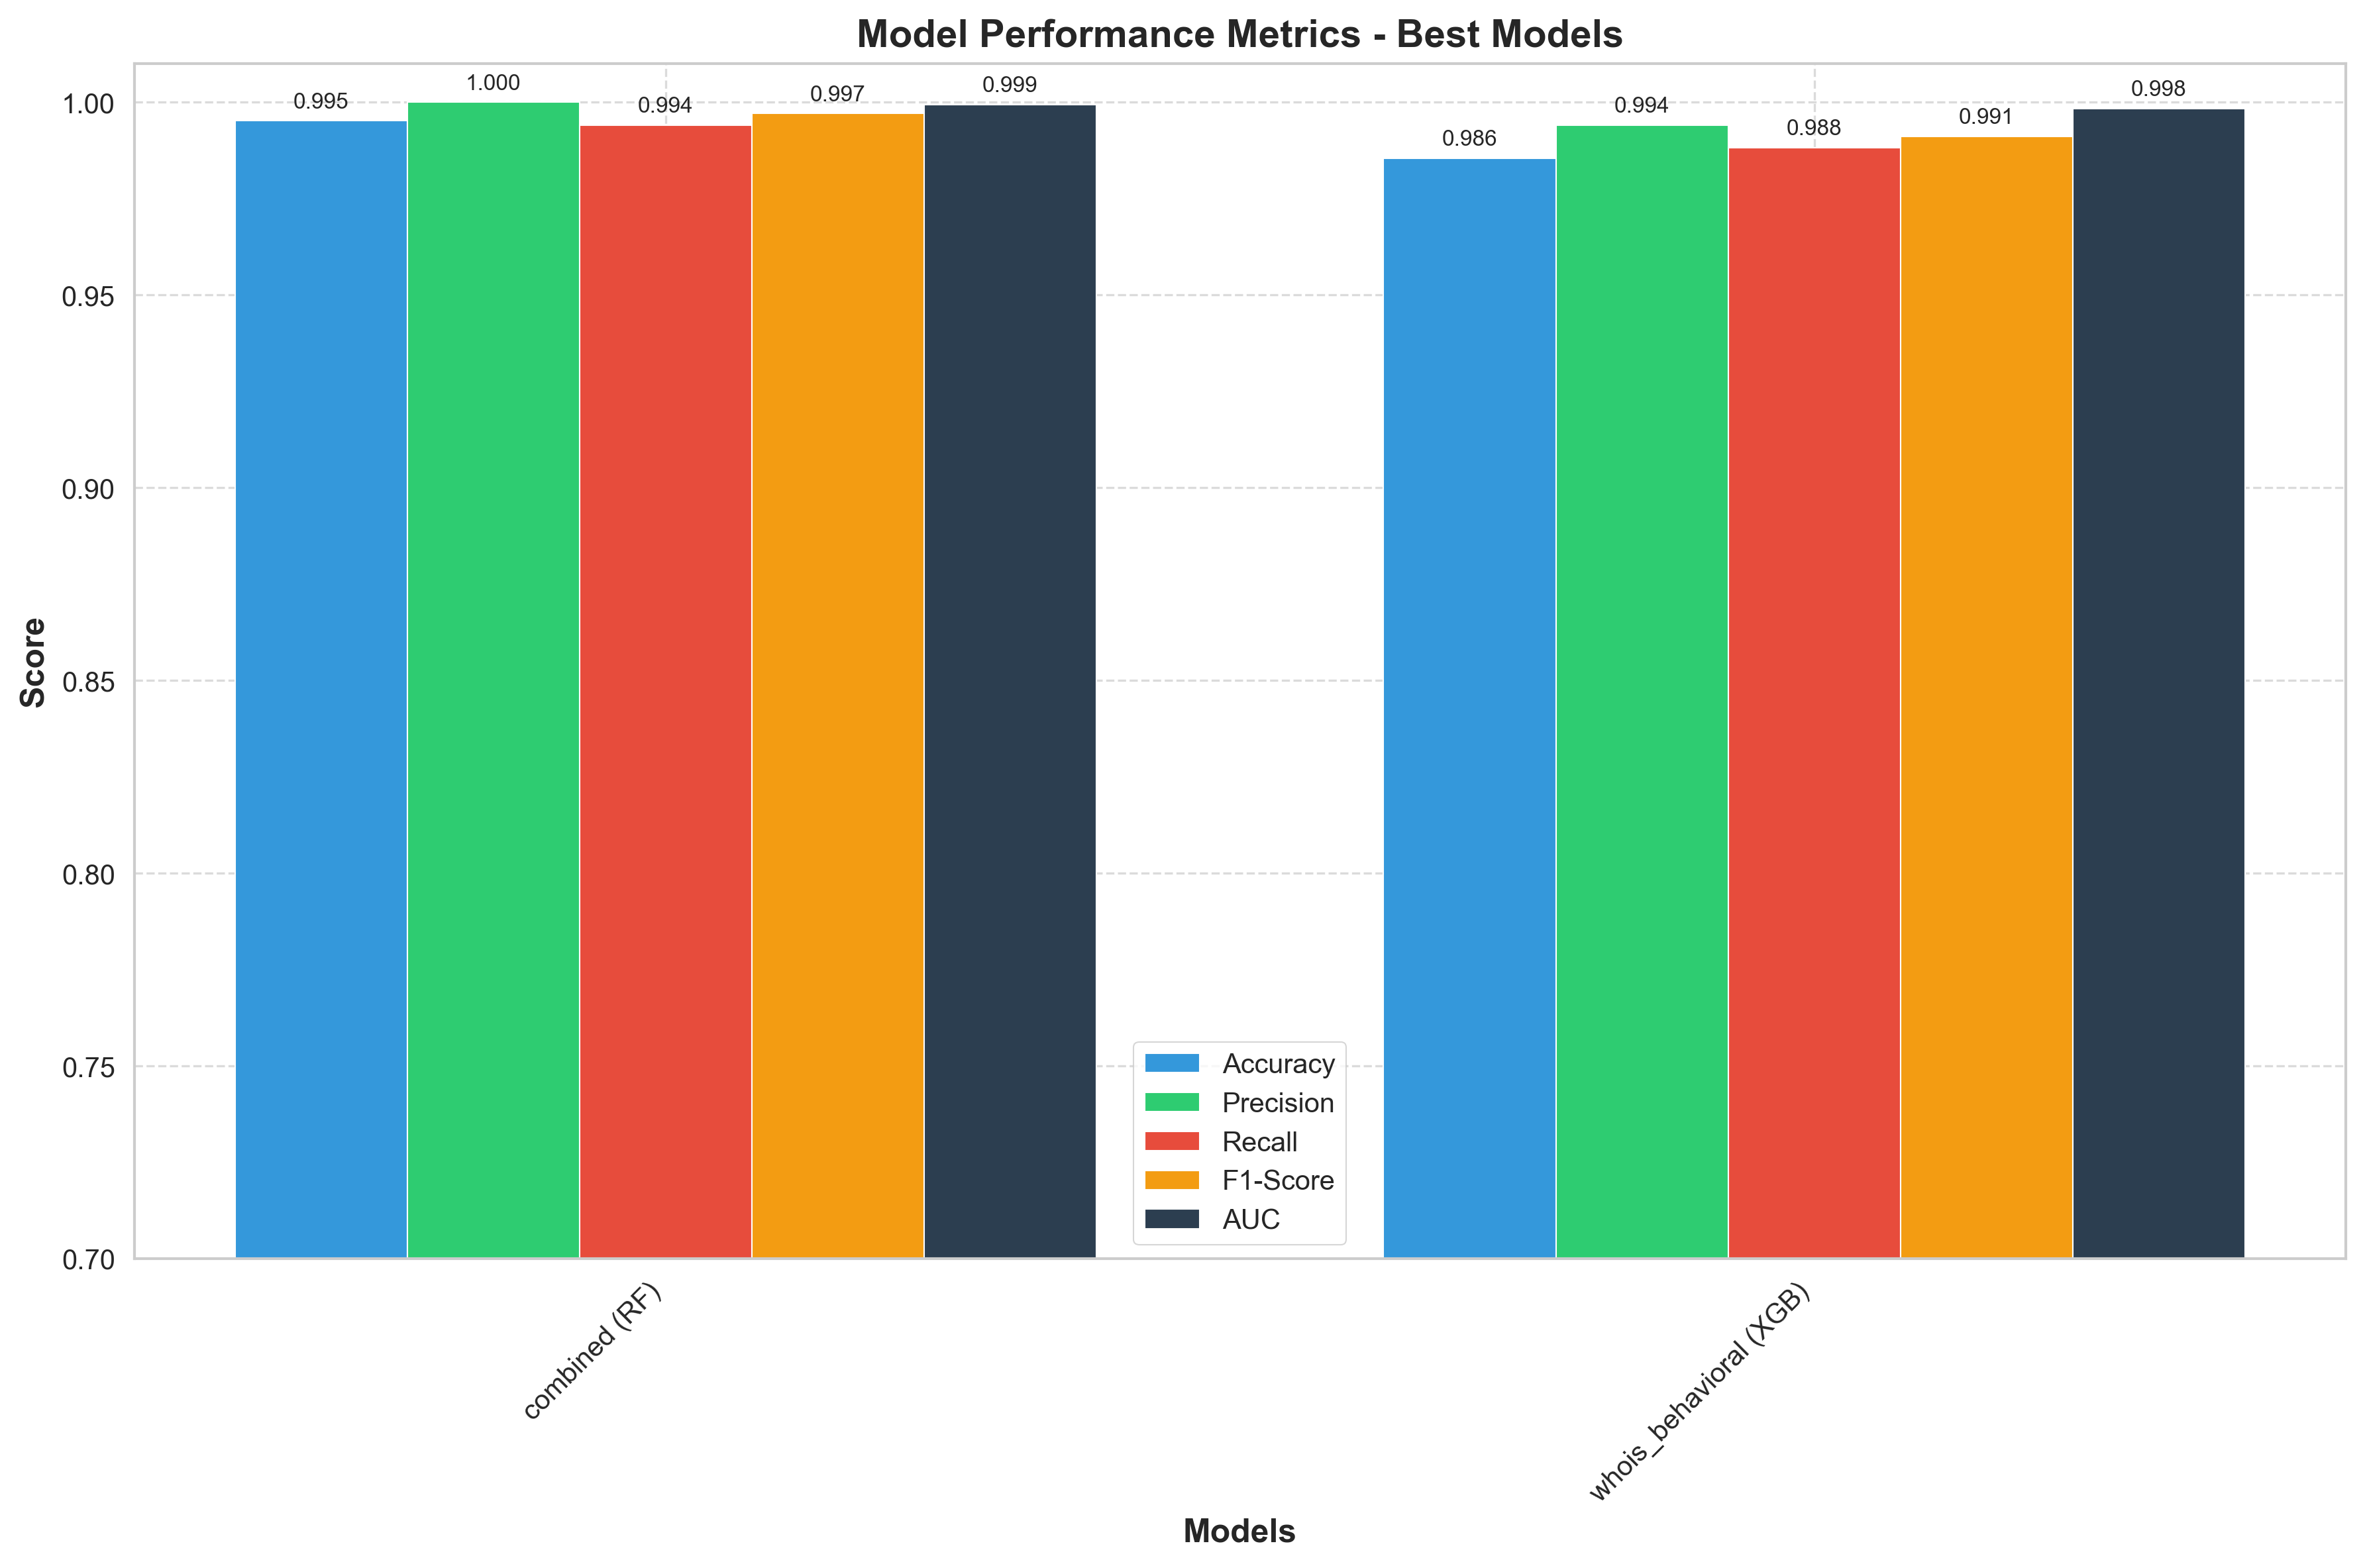
\includegraphics[width=0.9\columnwidth]{image/model_comparison_best_models.png}}
\caption{Comparison of Best Performing Models}
\label{fig:best_models}
\end{figure}

Our results indicate that the Random Forest model using all features achieved the highest accuracy (99.52\%), followed closely by the Random Forest model using WHOIS and Behavioral features (97.10\%). Among XGBoost models, the WHOIS + Behavioral combination performed best with 98.55\% accuracy.

\subsection{ROC Curve Analysis}
Figure \ref{fig:roc} shows the Receiver Operating Characteristic (ROC) curves for different models, illustrating their ability to distinguish between legitimate and phishing URLs.

\begin{figure}[htbp]
\centerline{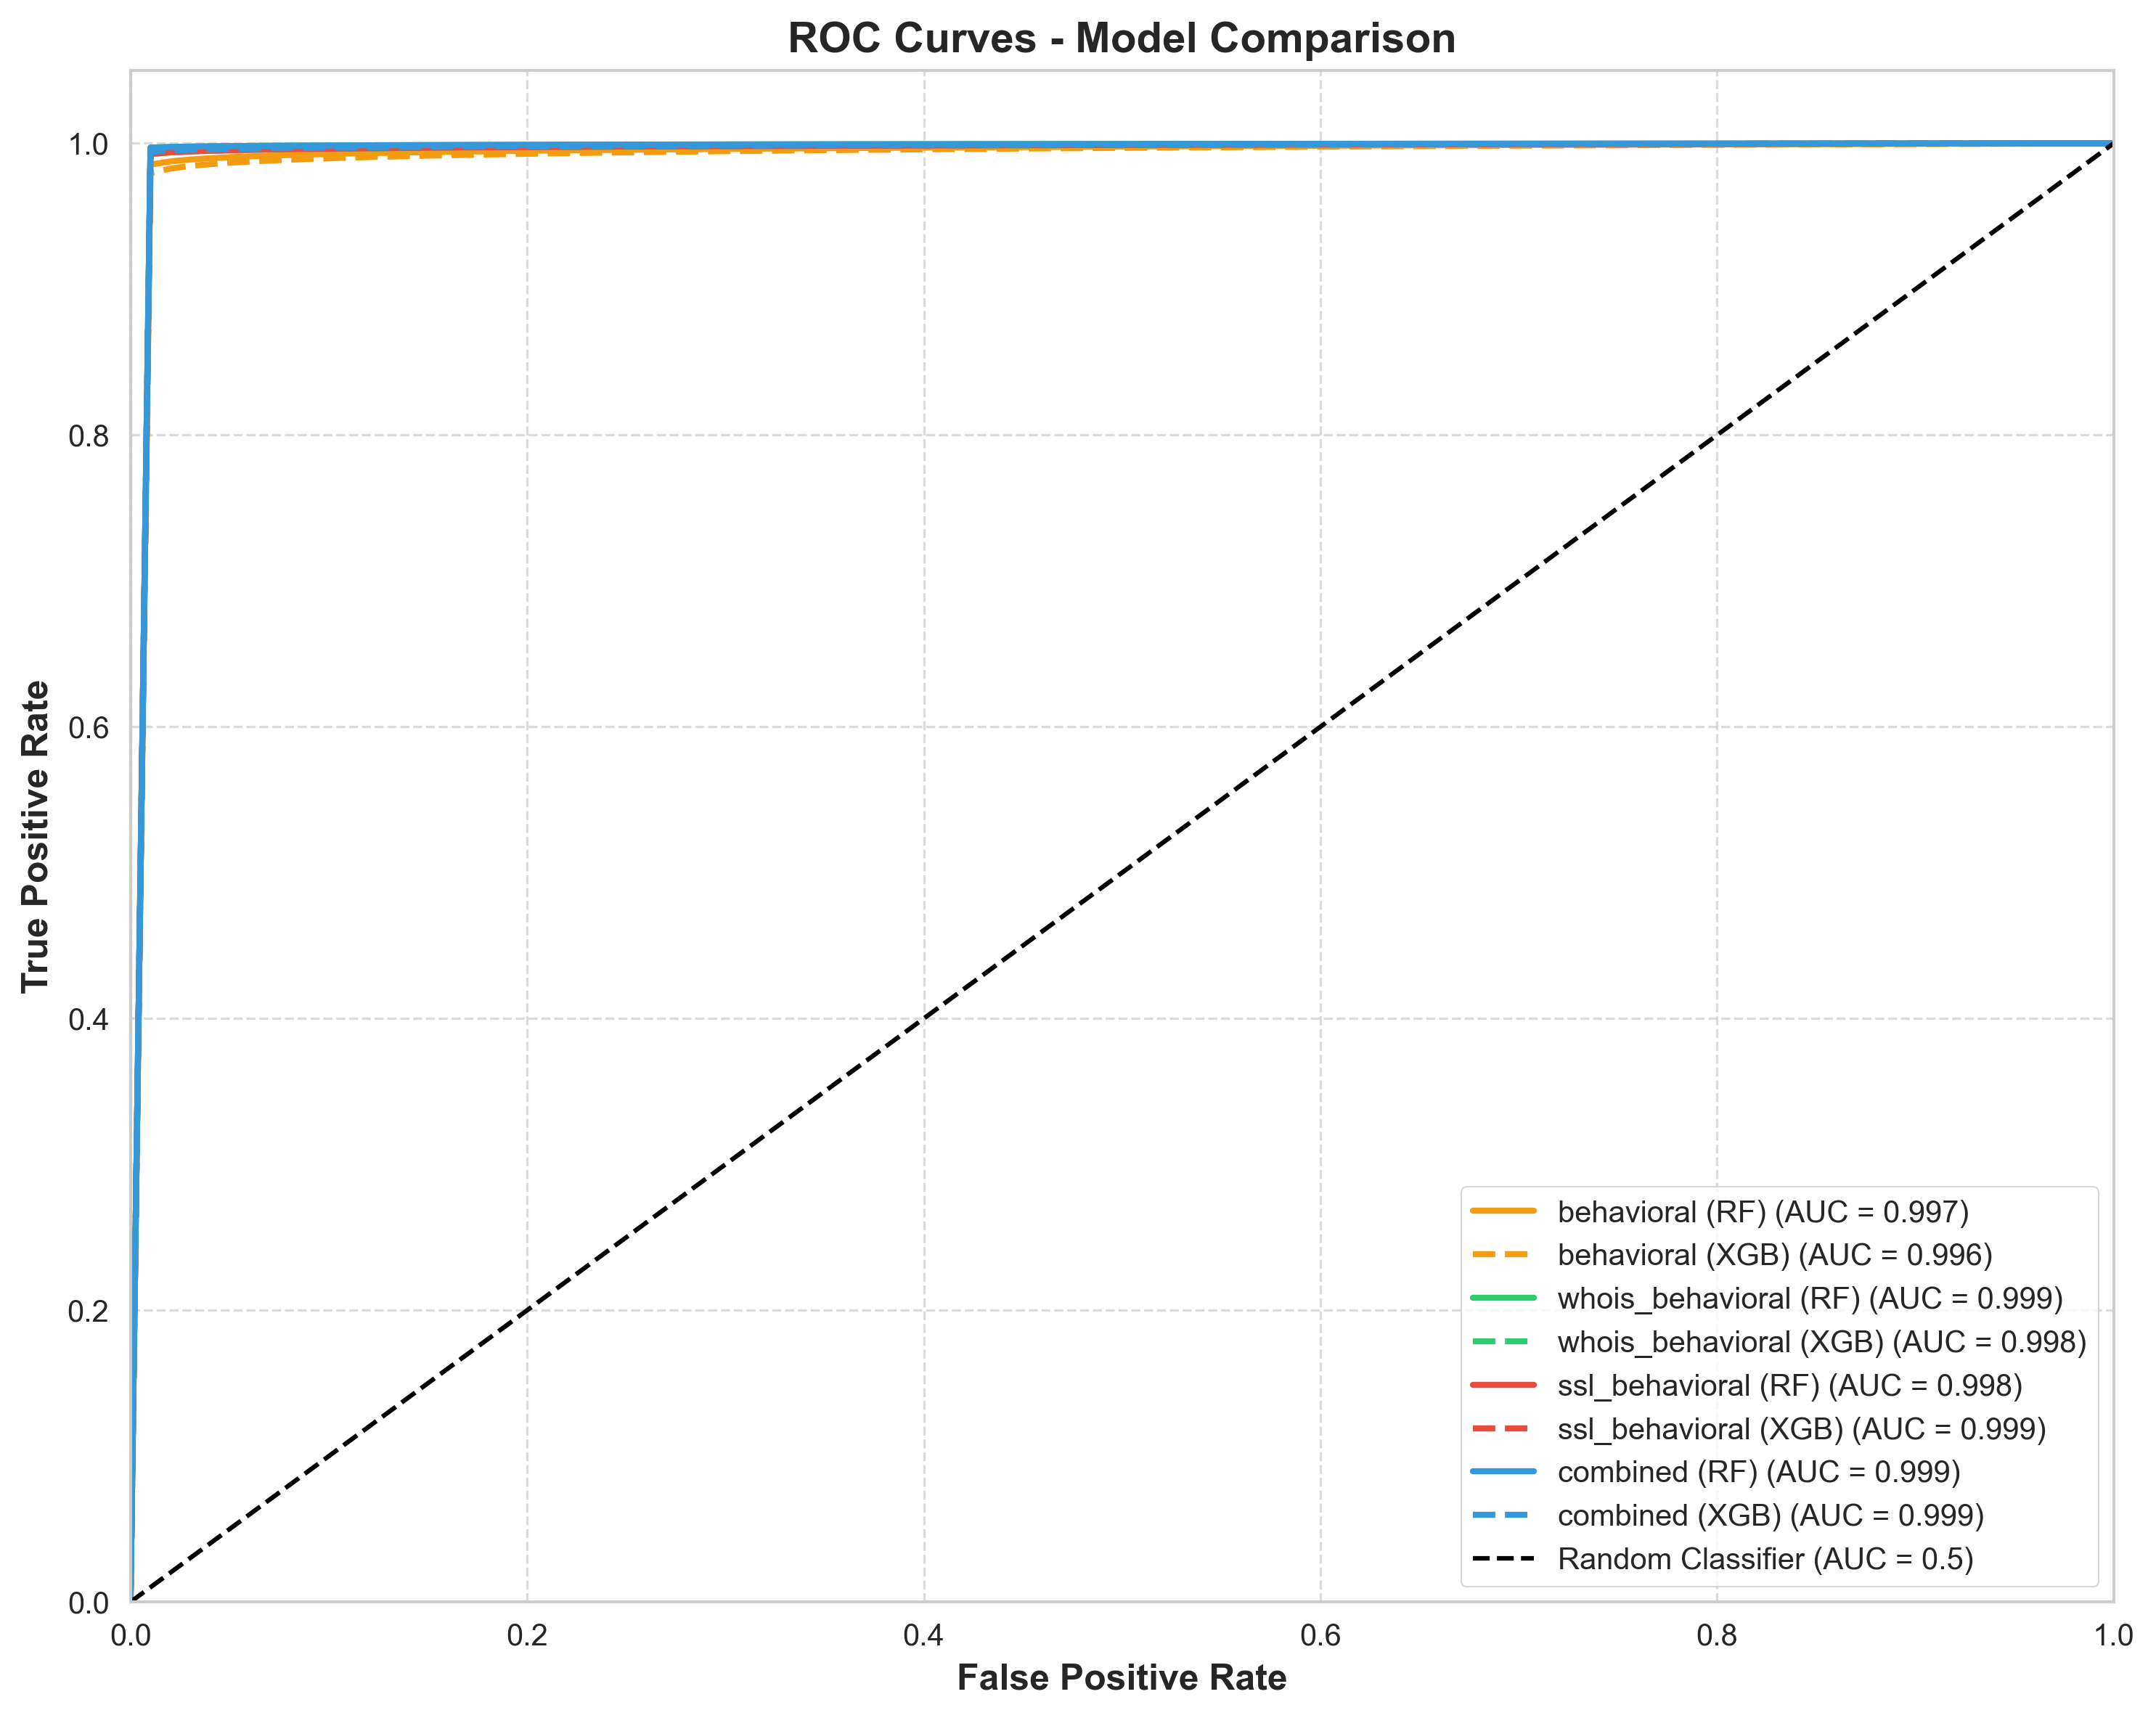
\includegraphics[width=0.9\columnwidth]{image/roc_curves.png}}
\caption{ROC Curves for Different Models}
\label{fig:roc}
\end{figure}

The area under the ROC curve (AUC) for our best model is 0.998, indicating excellent discriminative ability.

\subsection{Precision-Recall Analysis}
Given the imbalanced nature of phishing detection (where phishing URLs are typically the minority class), we also evaluated our models using precision-recall curves, as shown in Figure \ref{fig:pr_curve}.

\begin{figure}[htbp]
\centerline{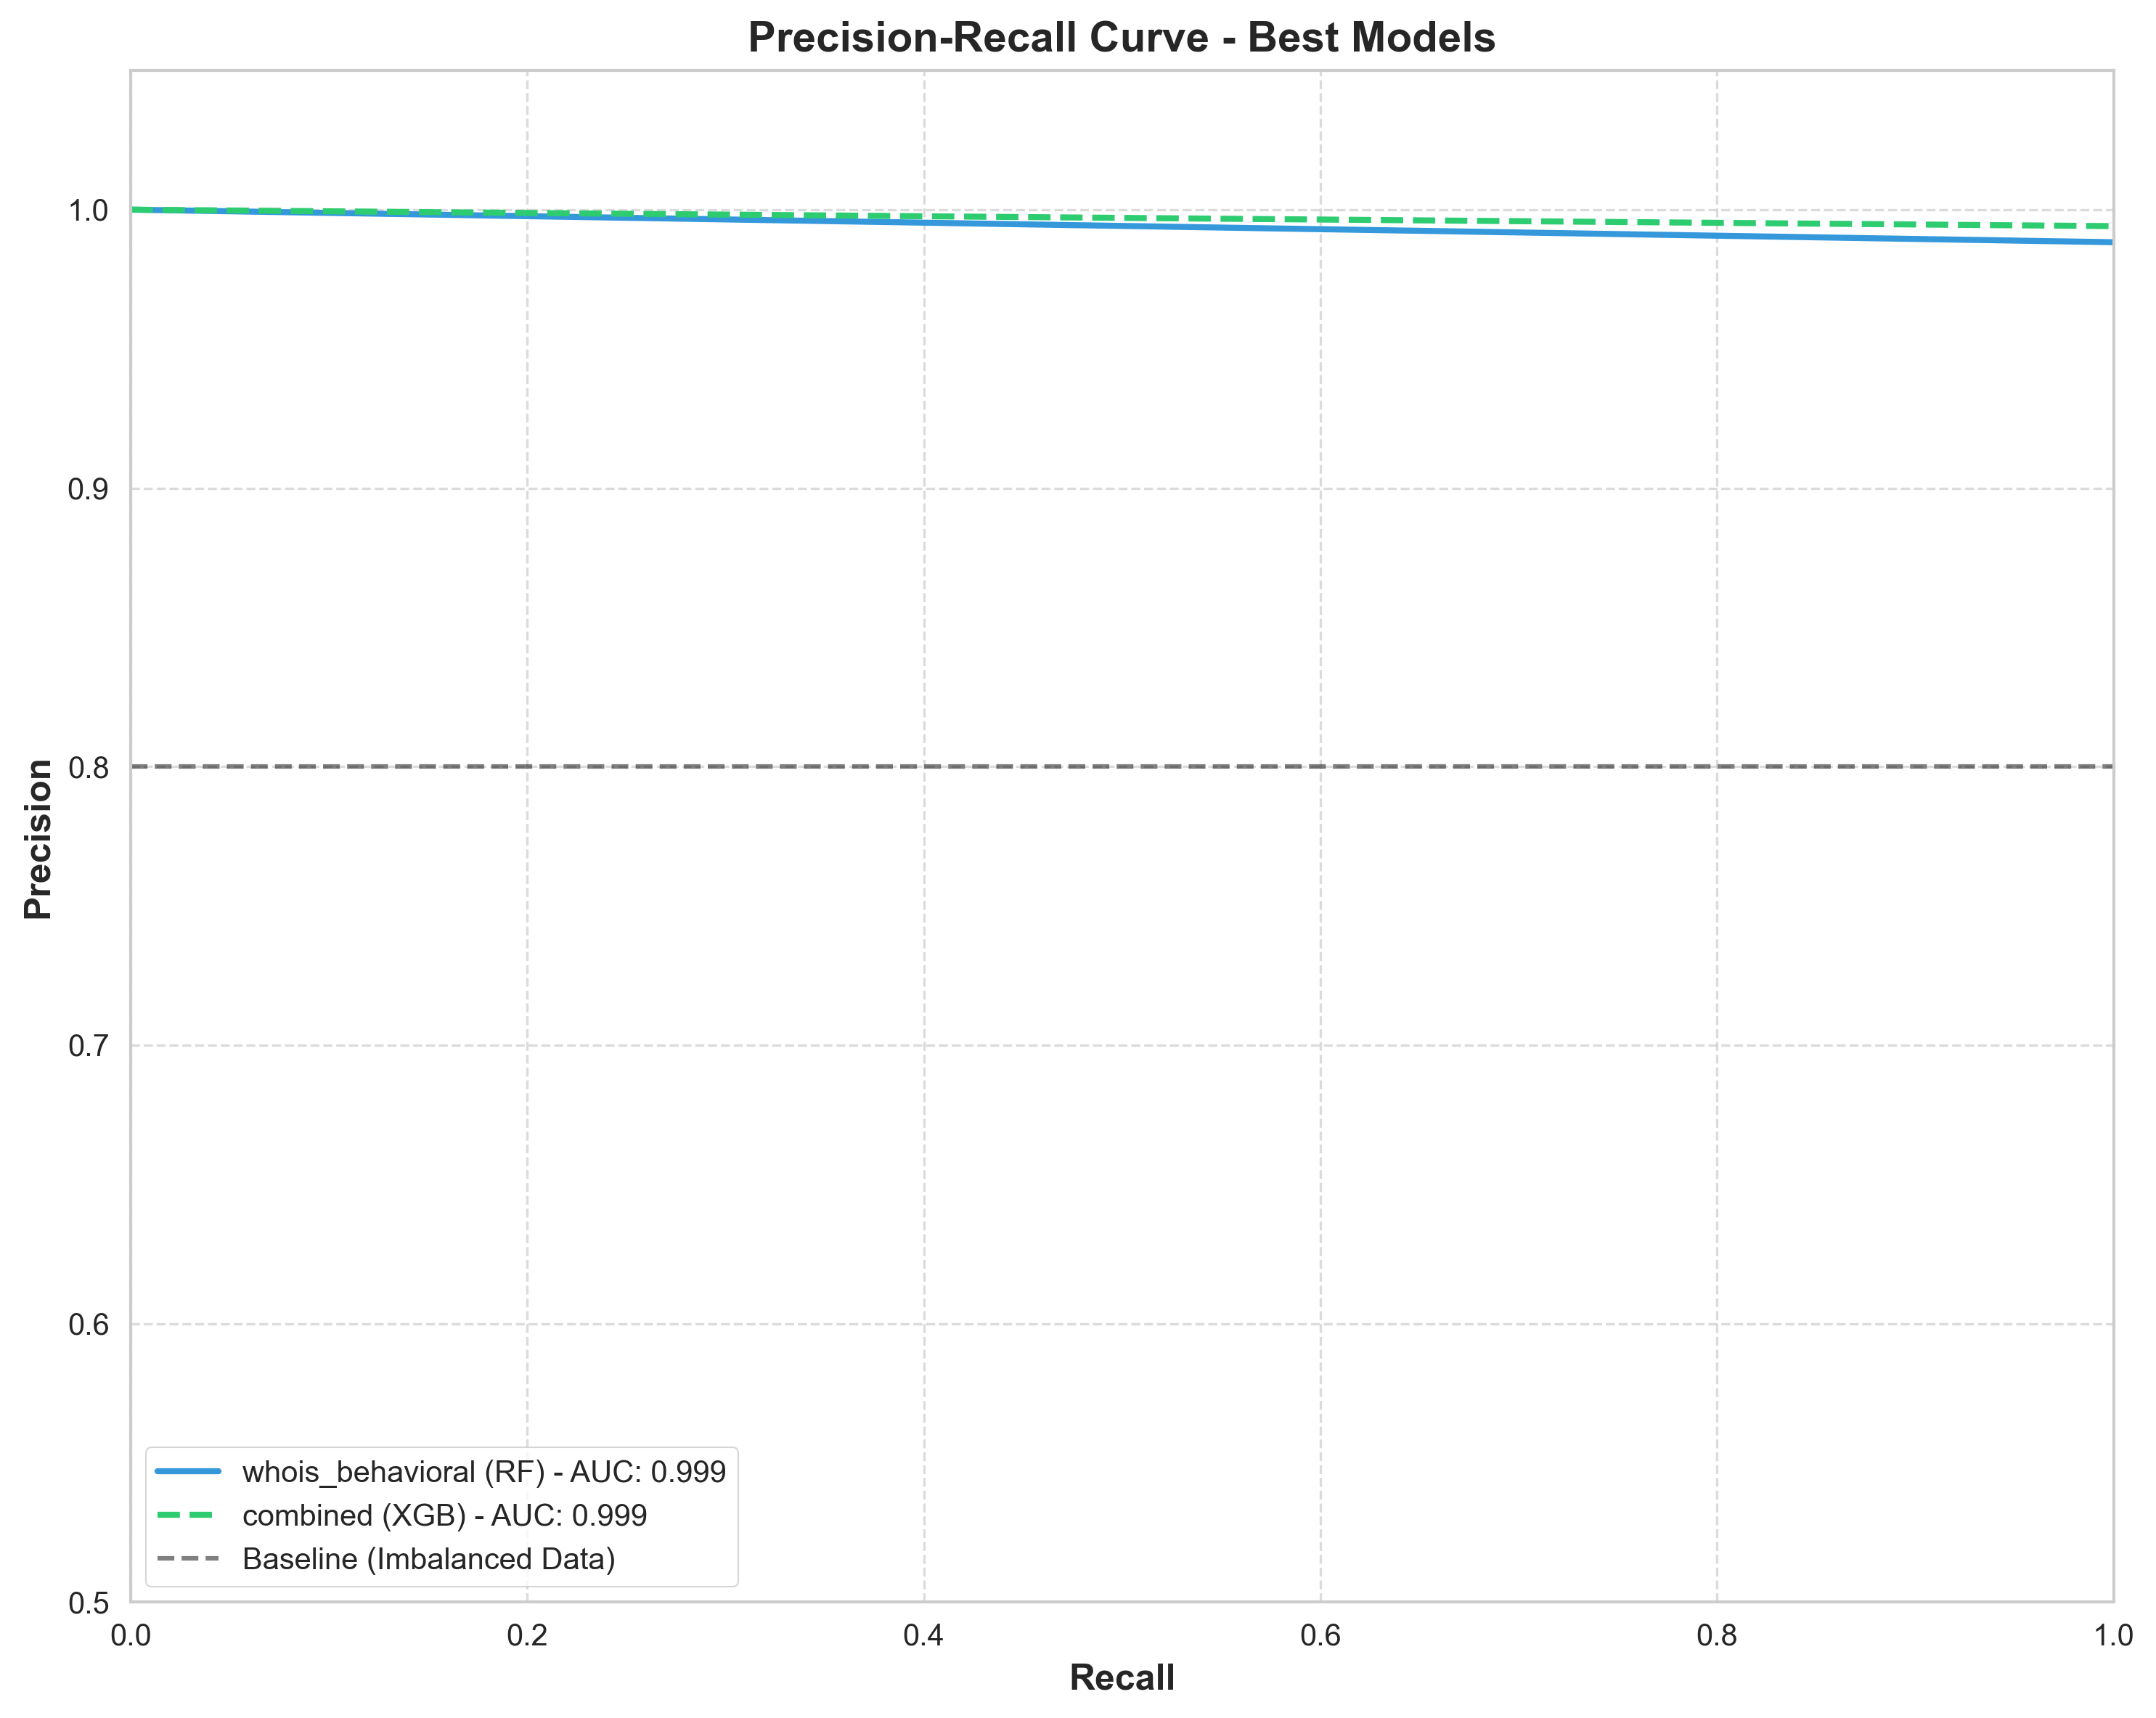
\includegraphics[width=0.9\columnwidth]{image/precision_recall_curve.png}}
\caption{Precision-Recall Curve}
\label{fig:pr_curve}
\end{figure}

\subsection{Confusion Matrix}
Figure \ref{fig:confusion} presents the confusion matrix for our best-performing model (Random Forest with all features).

\begin{figure}[htbp]
\centerline{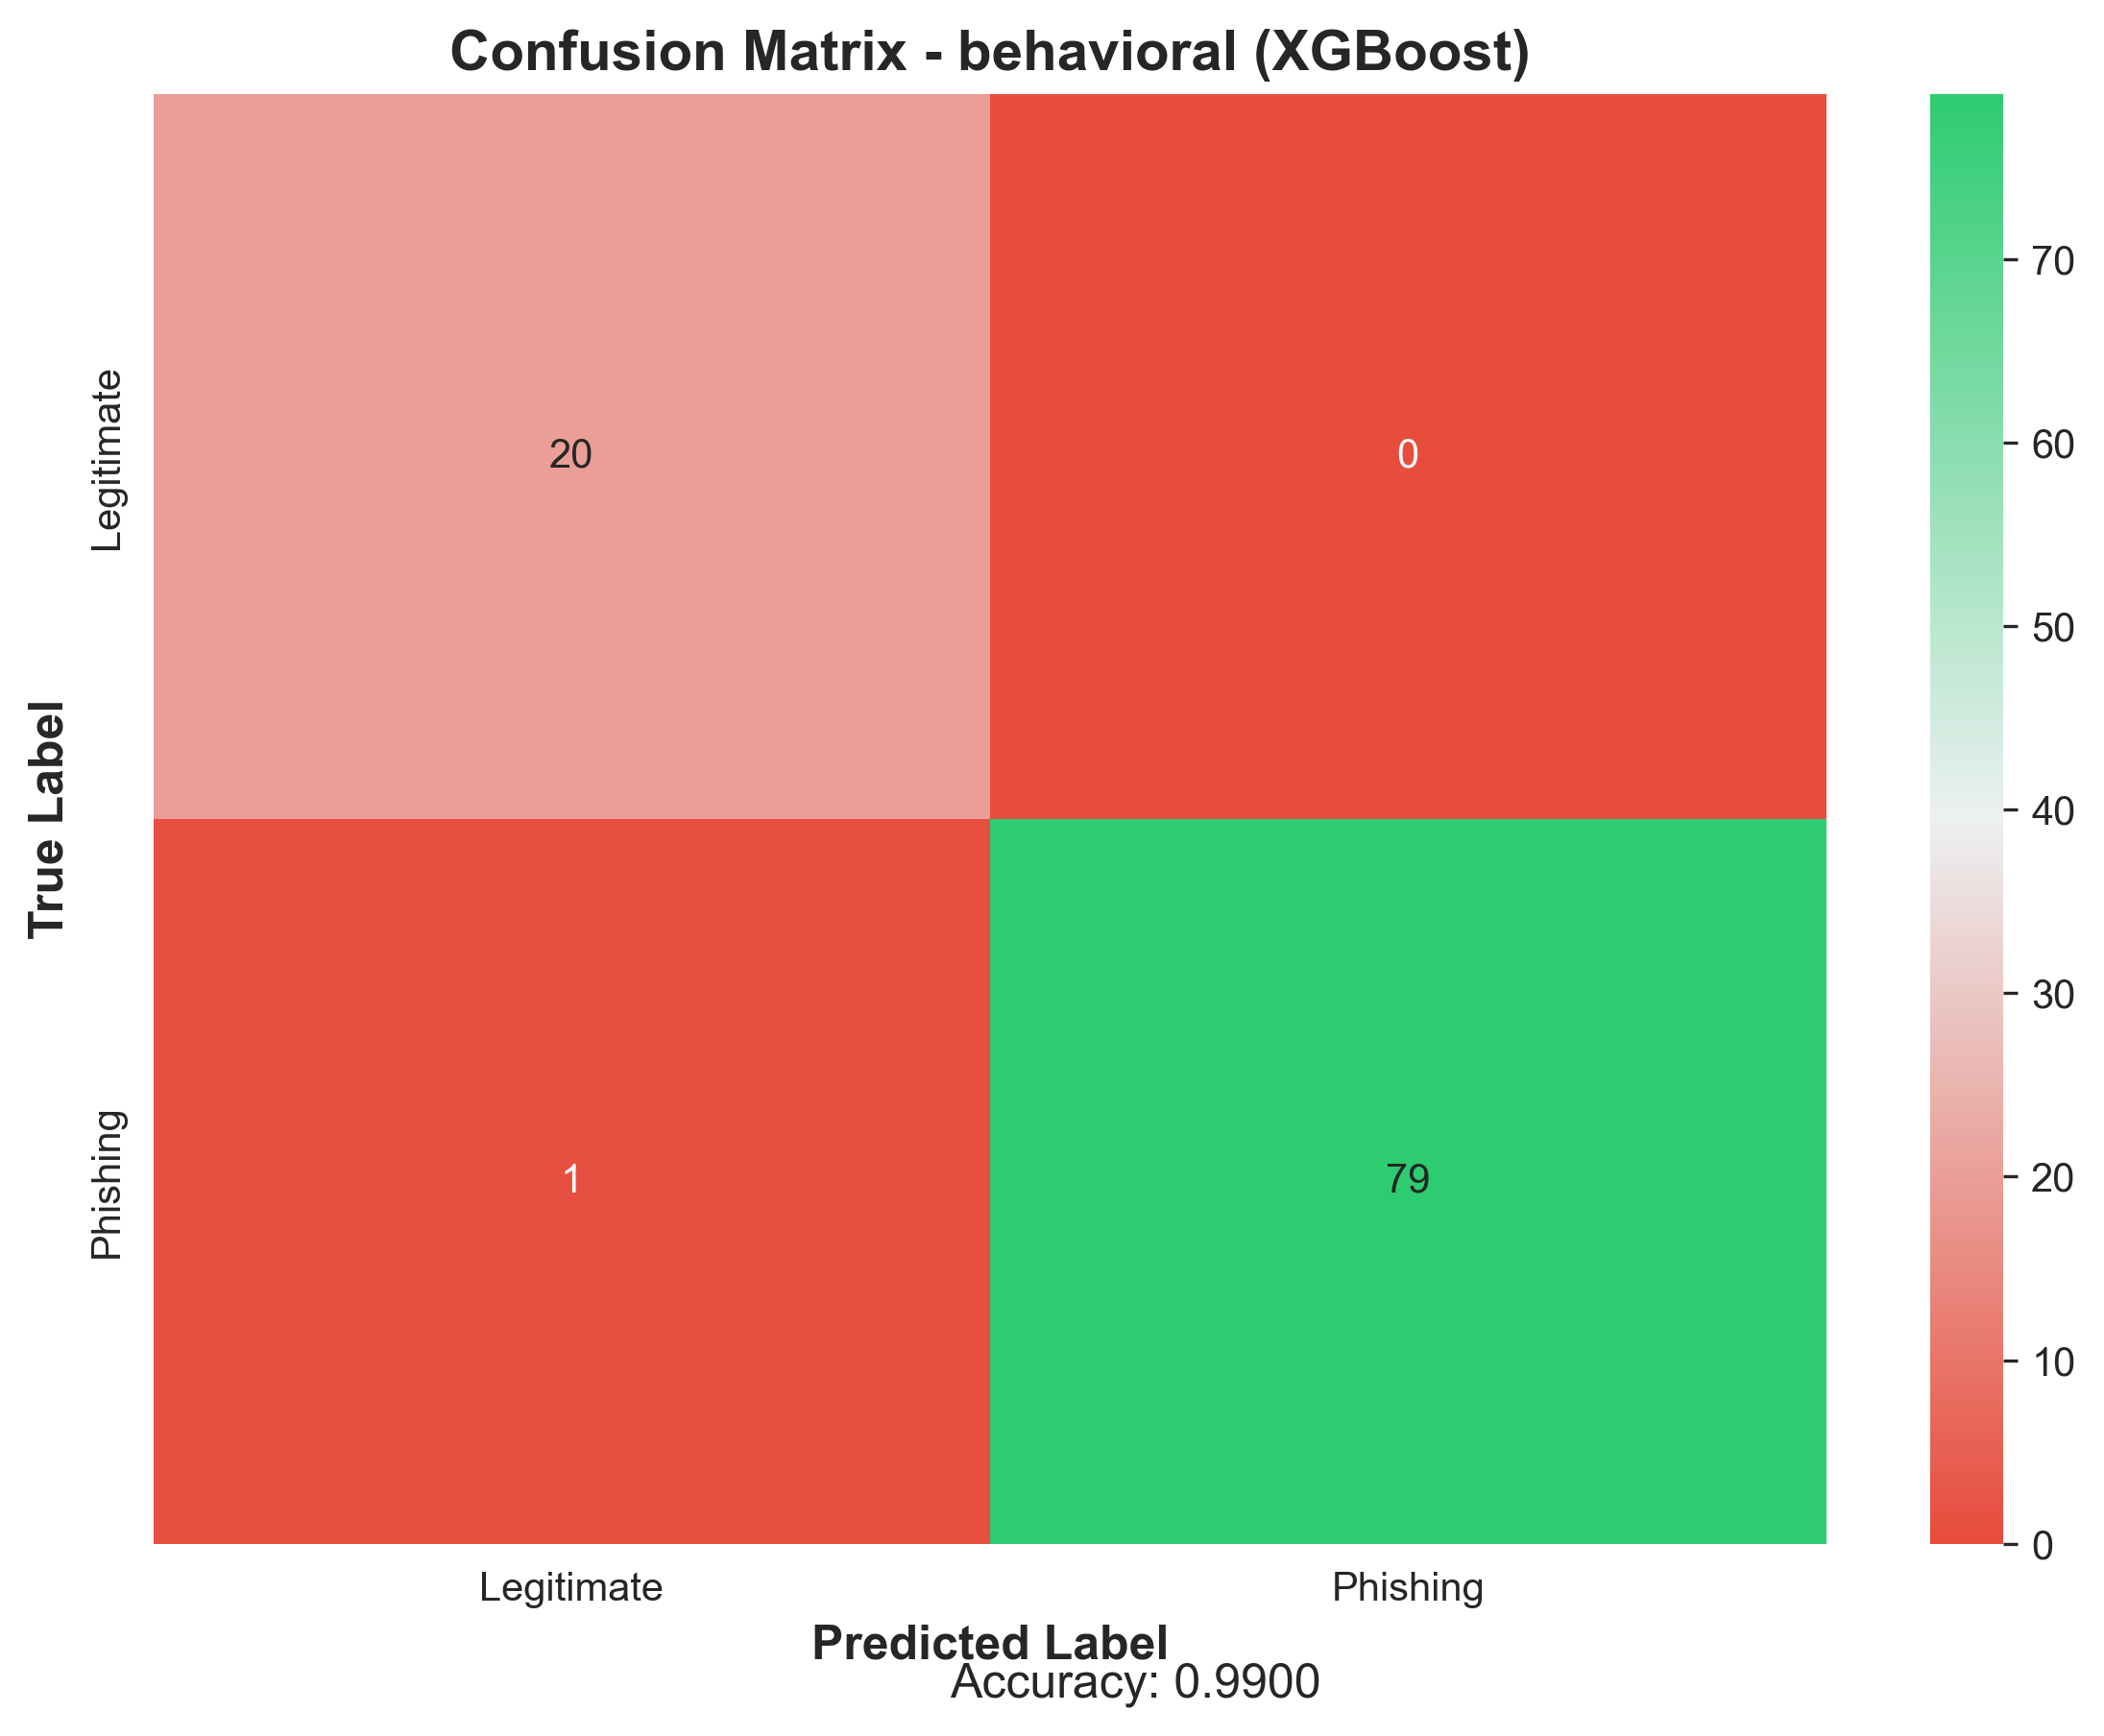
\includegraphics[width=0.9\columnwidth]{image/confusion_matrix.png}}
\caption{Confusion Matrix for Best Model}
\label{fig:confusion}
\end{figure}

The confusion matrix shows that our model achieves high precision and recall for both classes, with very few false positives and false negatives.

\subsection{Feature Importance}
To understand which features contribute most to the classification decision, we analyzed feature importance for our best model, as shown in Figure \ref{fig:importance}.

\begin{figure}[htbp]
\centerline{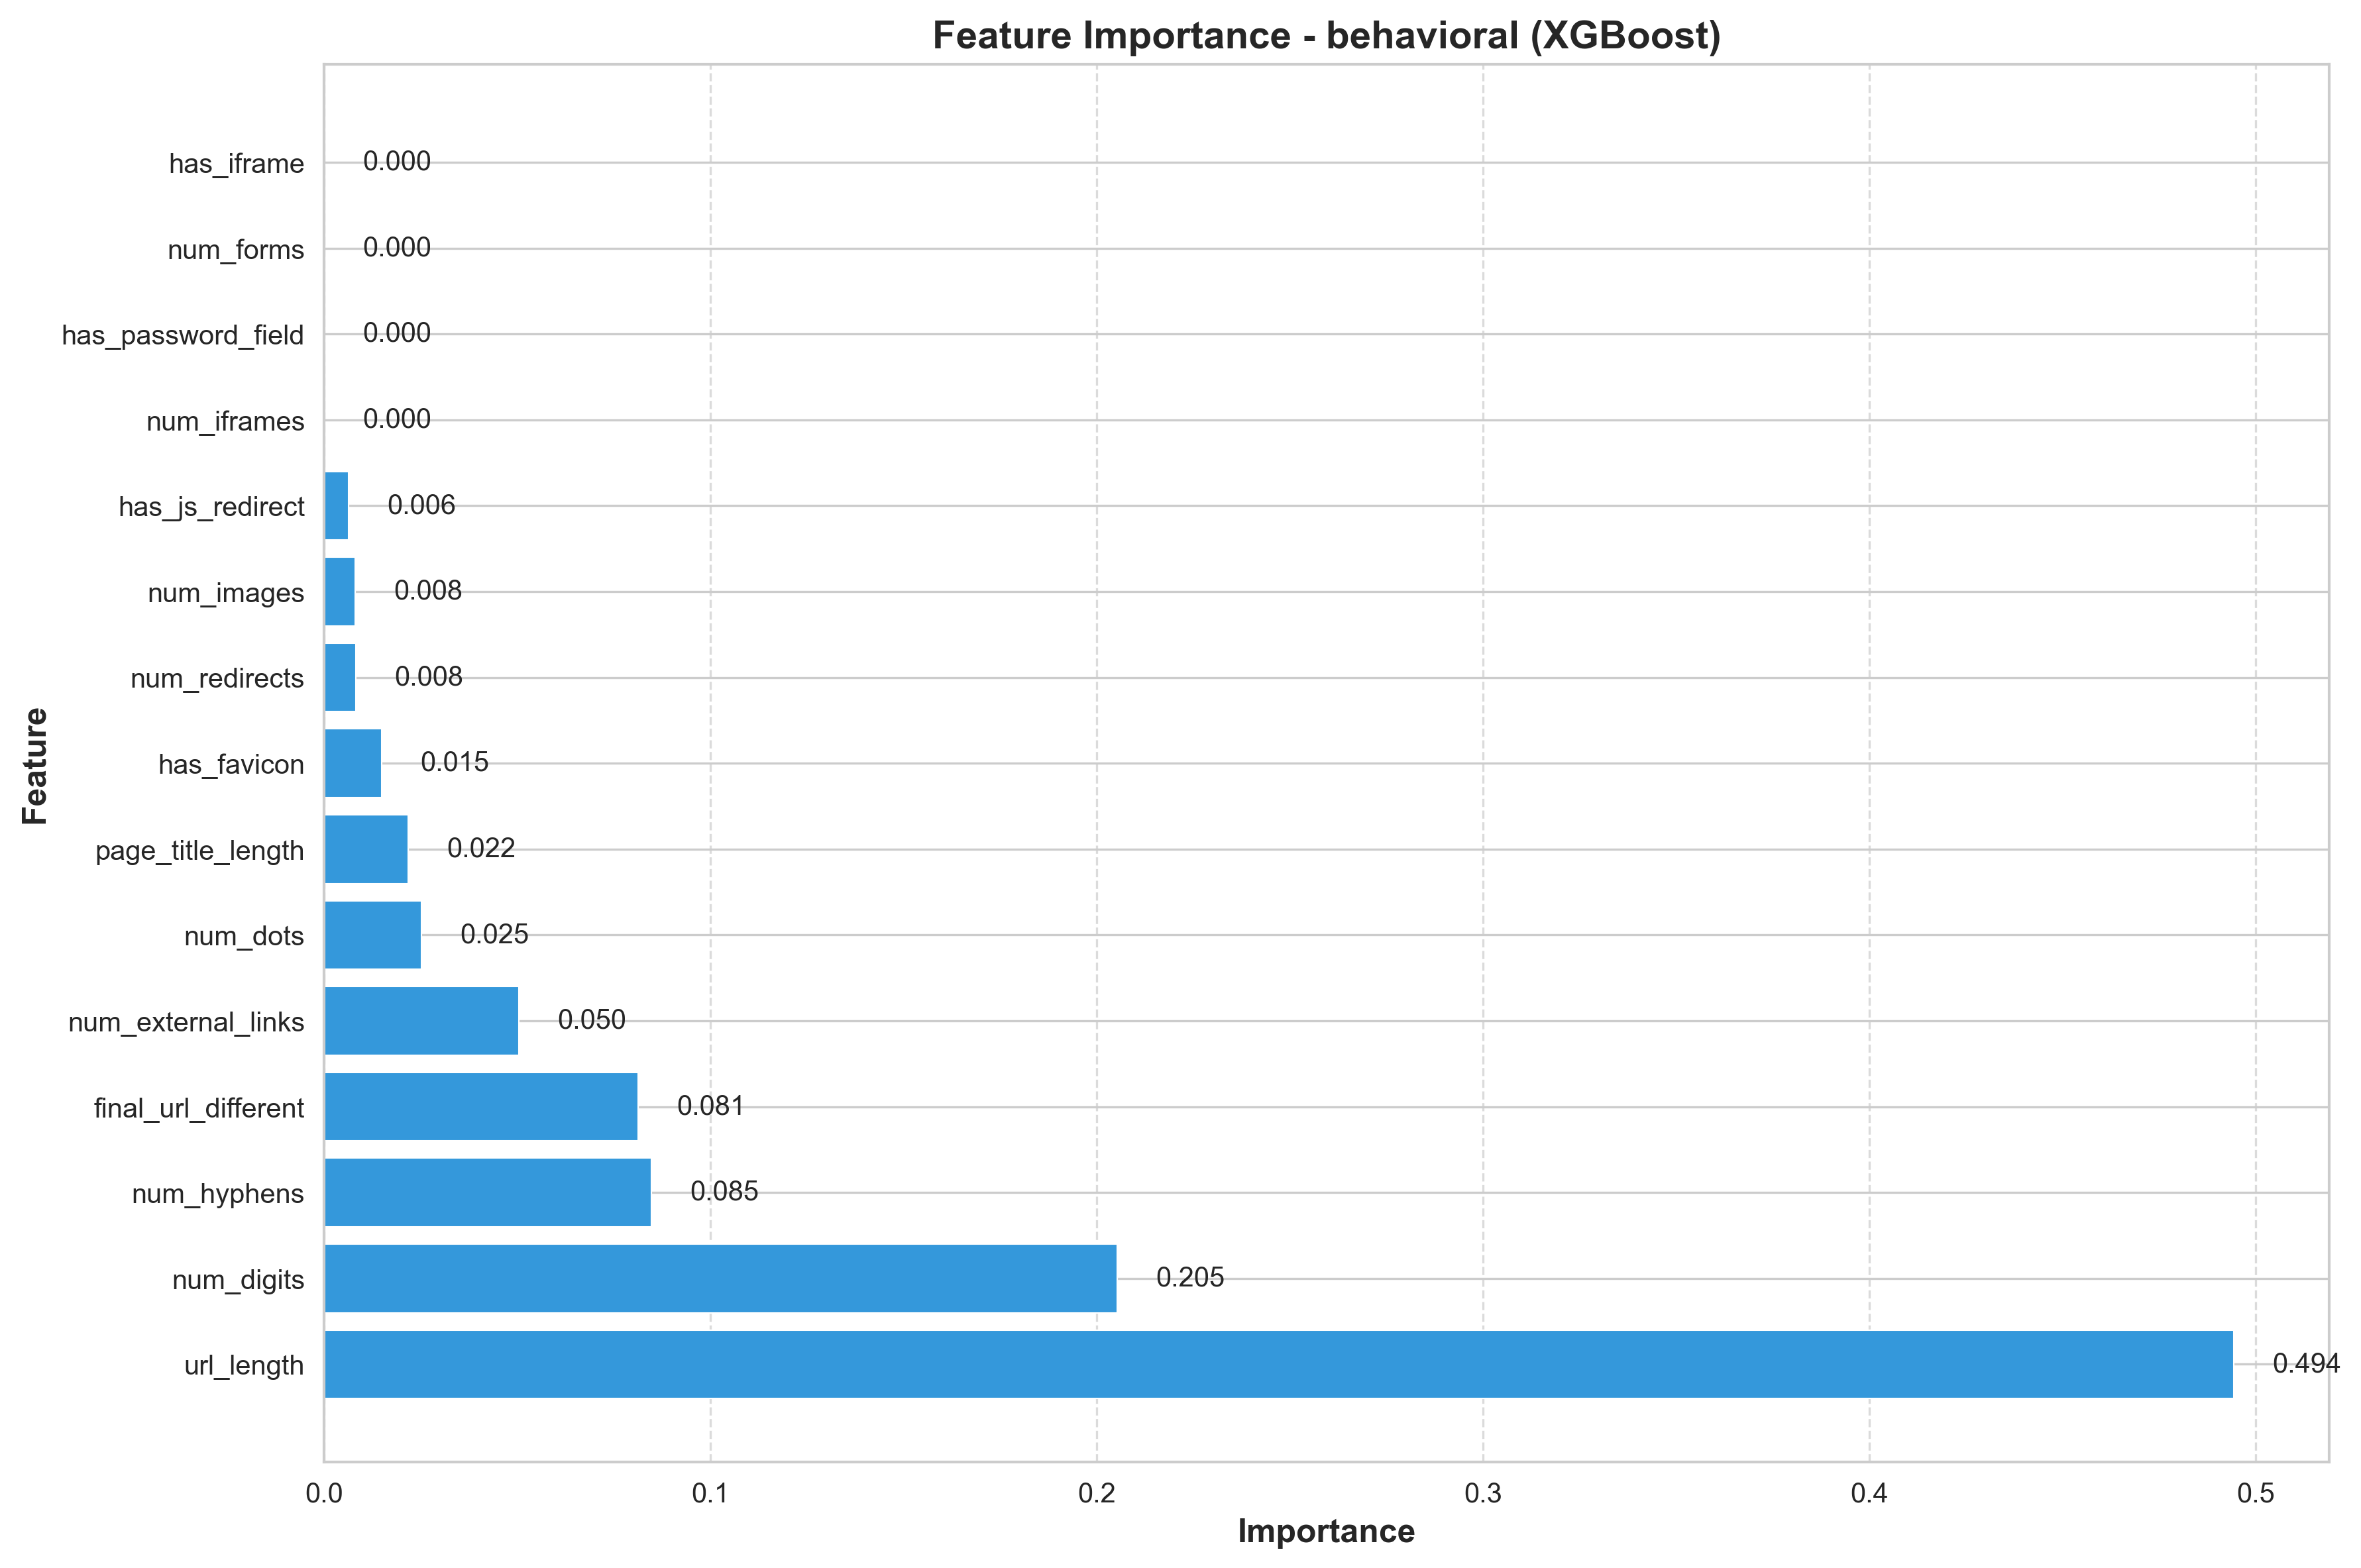
\includegraphics[width=0.9\columnwidth]{image/feature_importance.png}}
\caption{Feature Importance for Best Model}
\label{fig:importance}
\end{figure}

The analysis reveals that domain age, URL length, and SSL certificate validity period are among the most important features for phishing detection.

\section{Discussion}

\subsection{Performance Analysis}
Our experimental evaluation confirms that integrating multiple feature categories substantially enhances phishing detection performance compared to relying on a single set of attributes. As shown in Figure \ref{fig:rf_comparison} and Figure \ref{fig:xgb_comparison}, the Random Forest model leveraging all features achieved the highest accuracy (99.52\%), outperforming other combinations. This aligns with prior findings that ensemble approaches and multi-modal features provide robust detection capabilities \cite{frontiers2025multimodal, academia2022mlphishing}.

Interestingly, models trained exclusively on behavioral features (such as URL structure and lexical attributes) also produced strong performance, achieving 97.10\% with Random Forest and 98.07\% with XGBoost. This suggests that behavioral indicators are highly predictive, even in the absence of WHOIS or SSL metadata, which supports earlier work emphasizing URL-based heuristics as critical for phishing detection \cite{futureinternet2022behavior, academia2020cnn}.

Although XGBoost delivered competitive results—its best model (WHOIS + Behavioral) attained 98.55\% accuracy—Random Forest consistently showed more stable performance across different feature sets. This stability makes it a favorable candidate for practical deployment.

\subsection{Graceful Degradation}
One of the central strengths of our proposed framework is its capacity for \textit{graceful degradation}. In real-world scenarios, feature availability is often incomplete due to API rate limits, privacy restrictions, or evasion tactics by phishing actors. For example, SSL certificate information may not always be retrievable for certain domains. Our system addresses this challenge by dynamically falling back to alternative combinations such as WHOIS + Behavioral, which still achieved 97.10\% accuracy with Random Forest. This modular flexibility makes the framework resilient and practical for diverse operational environments, consistent with recommendations from adaptive security systems in the literature \cite{acm2024features, irep2025benchmarking}.

\subsection{Feature Importance Analysis}
To further interpret the model's decisions, we analyzed feature importance for the best-performing model, illustrated in Figure \ref{fig:importance}. The analysis reveals several key insights:

\begin{enumerate}
    \item \textbf{Domain Age:} Newly registered domains are strongly correlated with phishing activity, consistent with trends reported in prior work \cite{systlitchange2023, arxiv2024featureimportance}.
    \item \textbf{URL Characteristics:} Attributes such as length, entropy, and presence of special characters provide strong discriminative signals \cite{futureinternet2022behavior}.
    \item \textbf{SSL Certificate Properties:} Features like certificate validity period and issuer reliability enhance model precision, confirming findings in SSL-based phishing studies \cite{mdpi2023deeplearning}.
    \item \textbf{Multi-Feature Synergy:} The integration of WHOIS, SSL, and behavioral signals creates a layered detection system that is harder for attackers to bypass \cite{frontiers2025multimodal}.
\end{enumerate}

\subsection{Limitations and Future Work}
While the framework demonstrates high performance, several limitations remain:

\begin{enumerate}
    \item \textbf{Dynamic Content Analysis:} Current models do not consider webpage visual or textual content, which could enhance detection against sophisticated spoofing \cite{academia2021urltran}.
    \item \textbf{Adversarial Robustness:} Attackers may adapt through adversarial URL manipulations; thus, resilience testing is a priority for future work \cite{wikipedia2025adversarial, wired2021aipishing}.
    \item \textbf{Real-Time Efficiency:} Optimizing feature extraction for low-latency environments will be crucial for practical browser or network-level deployment \cite{mdpi2022improved}.
    \item \textbf{Continuous Learning:} Incorporating incremental updates will help maintain relevance against evolving phishing tactics \cite{wired2018ai}.
    \item \textbf{Explainability:} While feature importance analysis provides interpretability, expanding explainable AI methods (e.g., SHAP, LIME) could improve trust among end-users and security analysts \cite{wiley2022explainable, arxiv2024featureimportance}.
\end{enumerate}

\section{Conclusion}
This study introduced \textbf{PhishGuard}, a multi-layered machine learning framework that integrates WHOIS, SSL, and behavioral features for phishing URL detection. Experimental results show that the framework consistently outperforms single-feature approaches, with the best model achieving an accuracy of 99.52\% \cite{oni2024phishing, mdpi2022improved}.  

The modular design allows for graceful degradation in the absence of certain feature categories, making the system suitable for real-world applications \cite{acm2024features, irep2025benchmarking}. Furthermore, feature importance analysis highlights the relative contribution of WHOIS, SSL, and behavioral signals, supporting transparency and explainability \cite{wiley2022explainable, arxiv2024featureimportance}.  

Future research will focus on incorporating dynamic content analysis \cite{academia2021urltran}, strengthening adversarial robustness \cite{wikipedia2025adversarial}, optimizing runtime performance, enabling continuous learning \cite{wired2018ai}, and enhancing explainability for broader adoption in operational environments \cite{wiley2022explainable}. Our findings contribute to advancing practical, interpretable, and adaptive phishing detection solutions \cite{frontiers2025multimodal, academia2022mlphishing}.


\bibliographystyle{IEEEtran}
\bibliography{References}

\end{document}